\section{SceneGraphNode.h File Reference}
\label{SceneGraphNode_8h}\index{SceneGraphNode.h@{SceneGraphNode.h}}


\subsection{Detailed Description}
\begin{Desc}
\item[Author:]Troy Taillefer \end{Desc}


\begin{Desc}
\item[Date:]December 2, 2007 \end{Desc}
\begin{Desc}
\item[Version:]0.1 \end{Desc}


Definition in file {\bf SceneGraphNode.h}.

{\tt \#include $<$string$>$}\par
{\tt \#include \char`\"{}GraphTypes.h\char`\"{}}\par
{\tt \#include $<$ostream$>$}\par


Include dependency graph for SceneGraphNode.h:\nopagebreak
\begin{figure}[H]
\begin{center}
\leavevmode
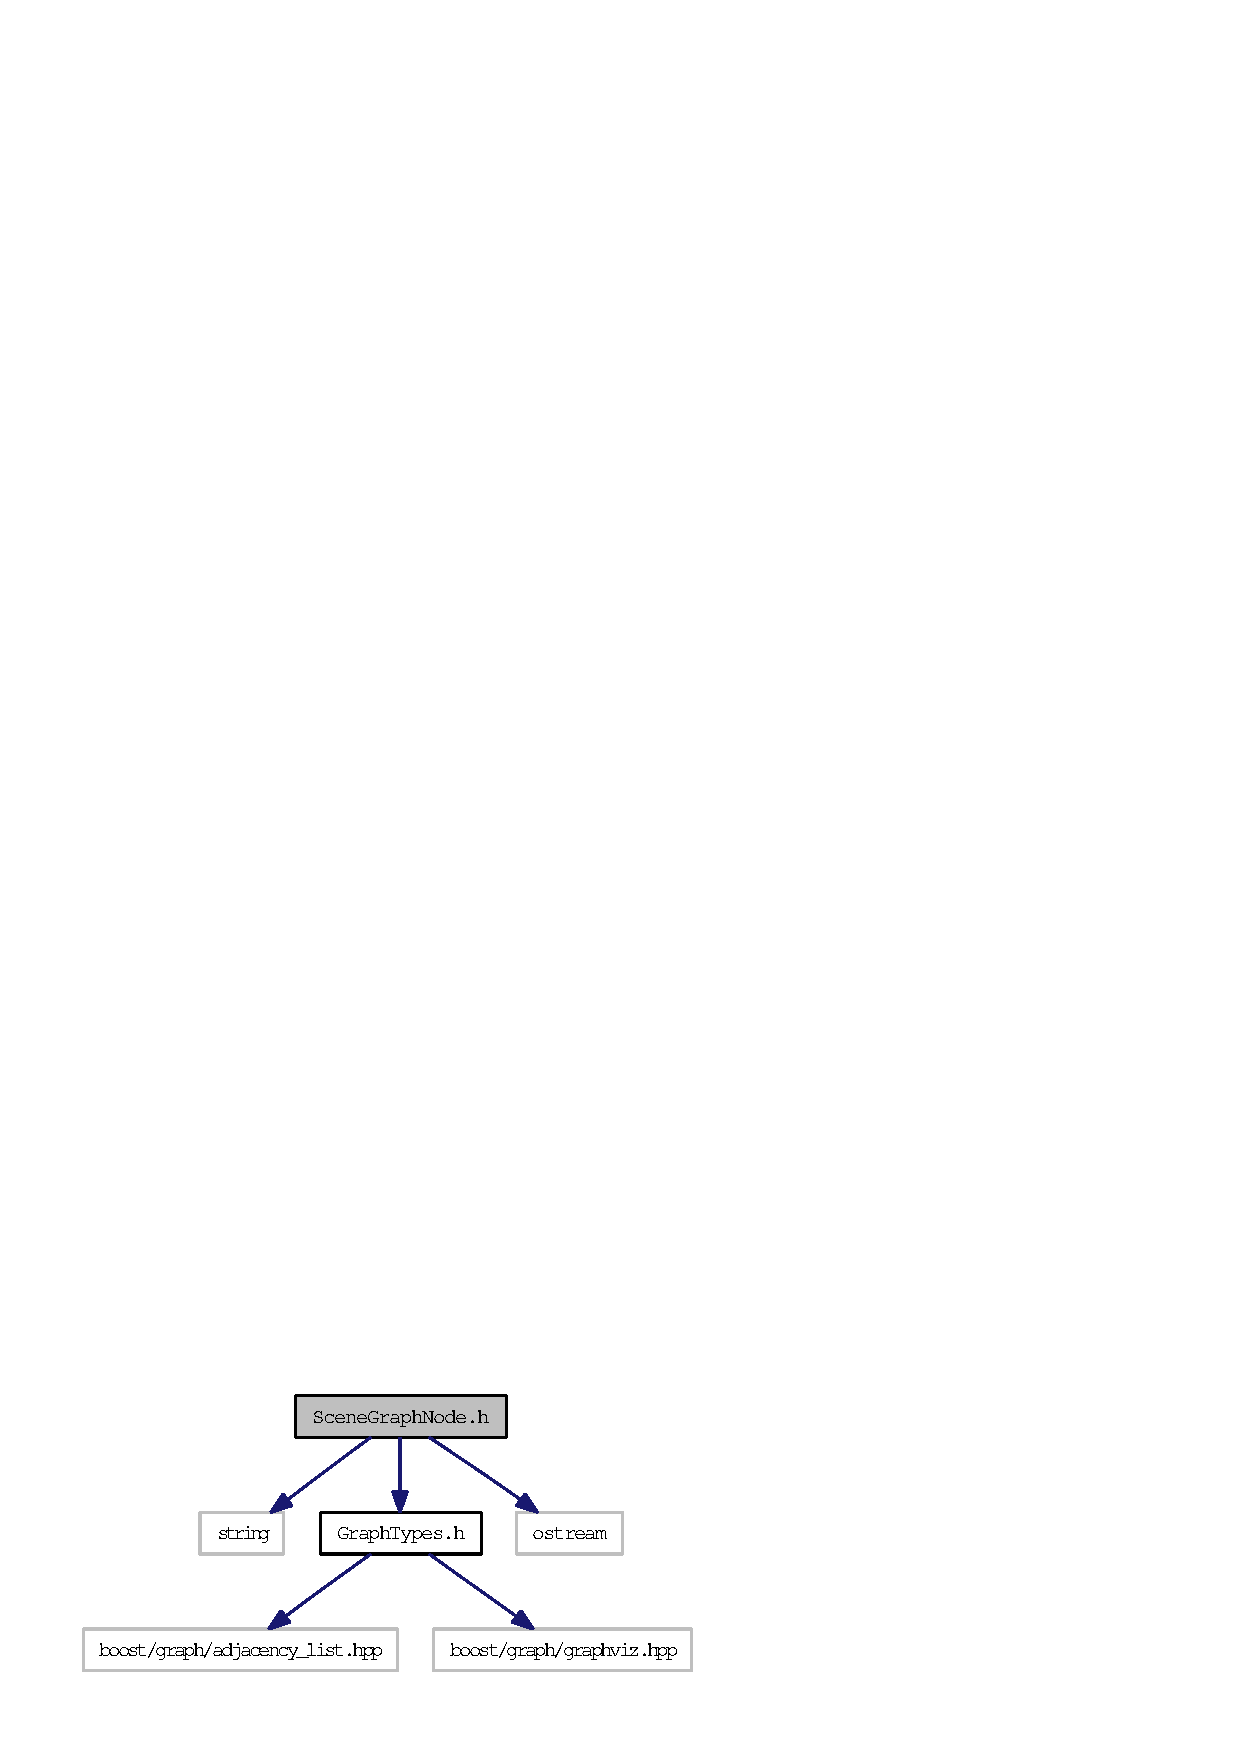
\includegraphics[width=168pt]{SceneGraphNode_8h__incl}
\end{center}
\end{figure}


This graph shows which files directly or indirectly include this file:\nopagebreak
\begin{figure}[H]
\begin{center}
\leavevmode
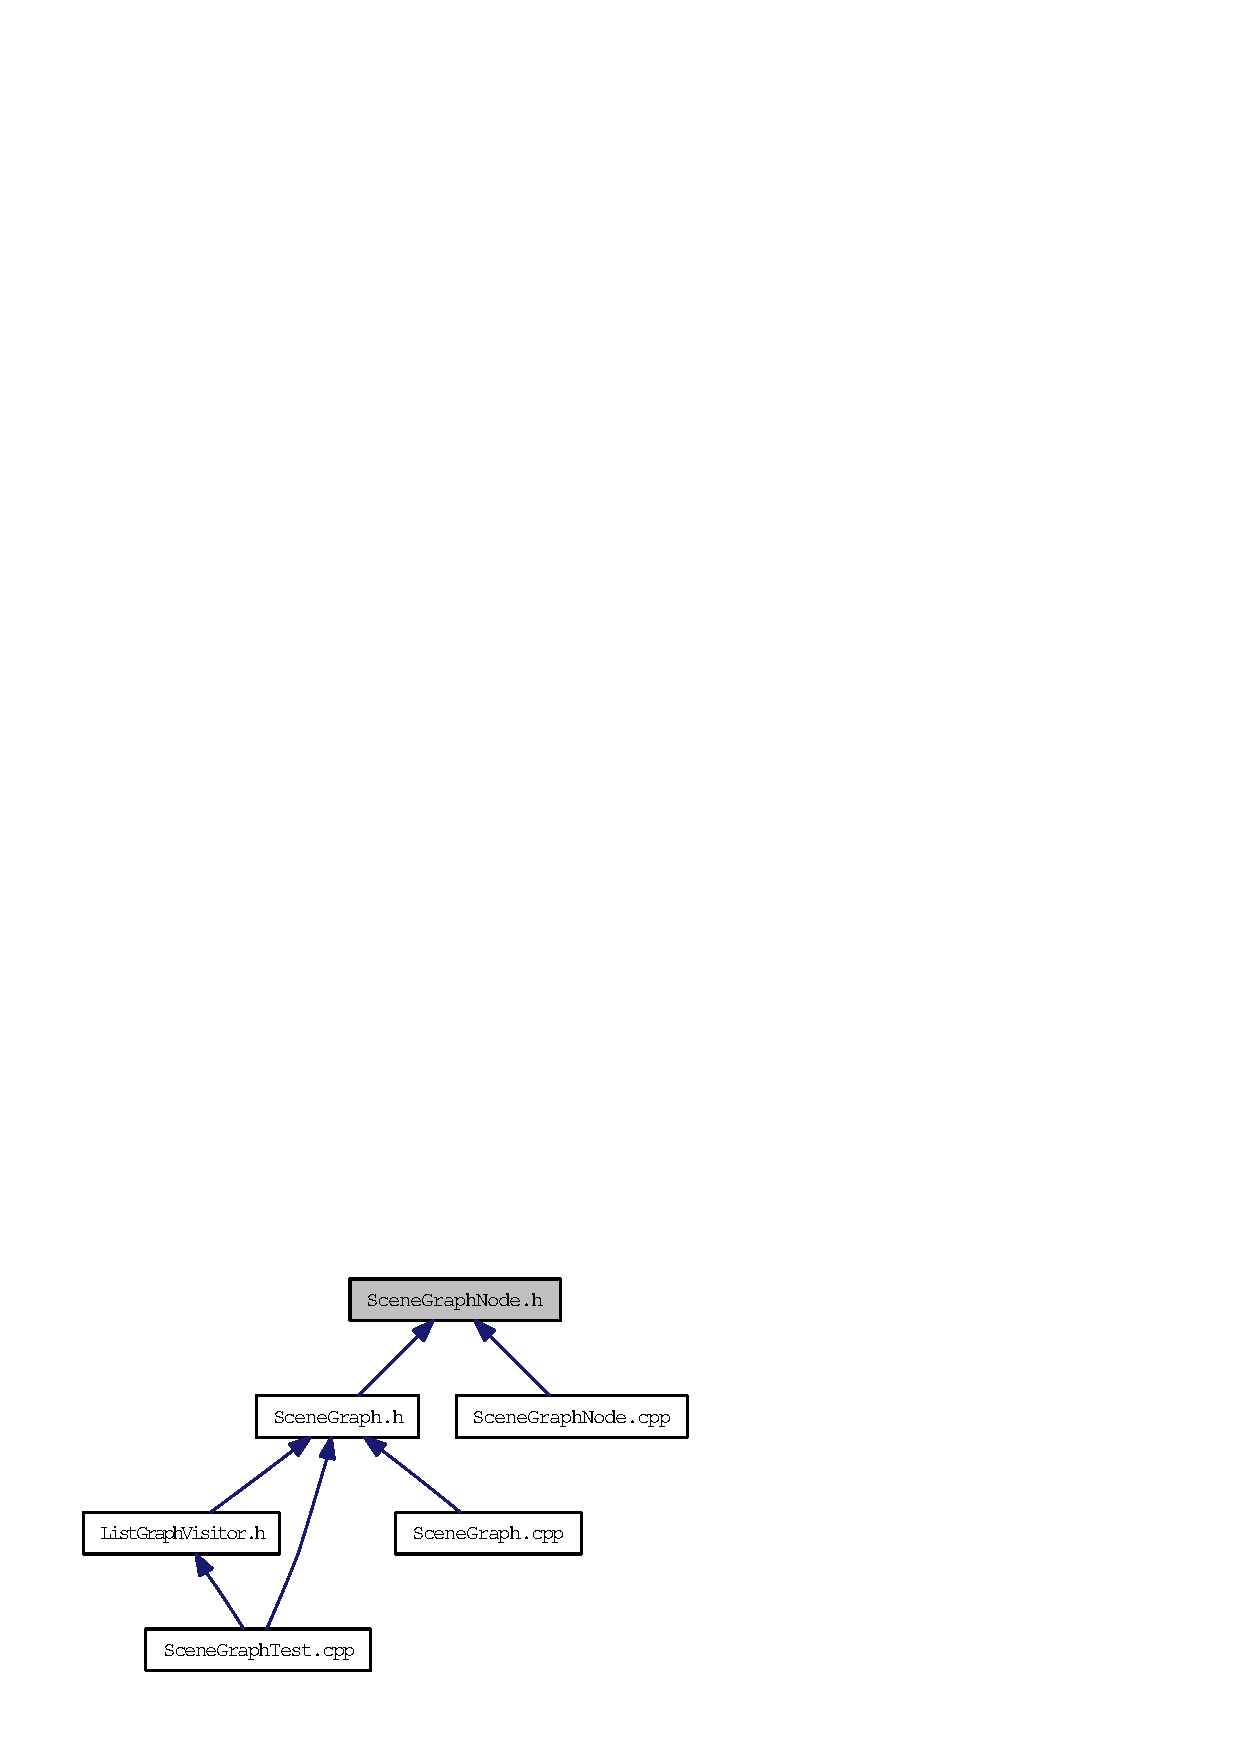
\includegraphics[width=166pt]{SceneGraphNode_8h__dep__incl}
\end{center}
\end{figure}
\subsection*{Data Structures}
\begin{CompactItemize}
\item 
class {\bf SceneGraphNode}
\begin{CompactList}\small\item\em This class is the base class for all the scene graph nodes. \item\end{CompactList}\end{CompactItemize}
